\documentclass[oneside,final,10pt]{article}

\listfiles               %  print all files needed to compile this document

\usepackage{relsize,makeidx,color,setspace,amsmath,amsfonts,amssymb}
\usepackage[table]{xcolor}
\usepackage{bm,ltablex,microtype}
\usepackage[pdftex]{graphicx}

\usepackage[T1]{fontenc}
%\usepackage[latin1]{inputenc}
\usepackage{ucs}
\usepackage[utf8x]{inputenc}

\usepackage{lmodern}         % Latin Modern fonts derived from Computer Modern

% Hyperlinks in PDF:
\definecolor{linkcolor}{rgb}{0,0,0.4}
\usepackage{hyperref}
\hypersetup{
    breaklinks=true,
    colorlinks=true,
    linkcolor=linkcolor,
    urlcolor=linkcolor,
    citecolor=black,
    filecolor=black,
    %filecolor=blue,
    pdfmenubar=true,
    pdftoolbar=true,
    bookmarksdepth=3   % Uncomment (and tweak) for PDF bookmarks with more levels than the TOC
    }

\setcounter{tocdepth}{2}  % levels in table of contents

\setcounter{topnumber}{2}
\setcounter{bottomnumber}{2}
\setcounter{totalnumber}{4}
\renewcommand{\topfraction}{0.95}
\renewcommand{\bottomfraction}{0.95}
\renewcommand{\textfraction}{0}
\renewcommand{\floatpagefraction}{0.75}
\clubpenalty = 10000
\widowpenalty = 10000

\raggedbottom
\makeindex
\usepackage[totoc]{idxlayout}   % for index in the toc
\usepackage[nottoc]{tocbibind}  % for references/bibliography in the toc

\begin{document}

\thispagestyle{empty}

\begin{center}
{\LARGE\bf
\begin{spacing}{1.25}
Computing Across the Disciplines: Study Programs in Computational Science and Data Science
\end{spacing}
}
\end{center}

\begin{center}
{\bf A comprehensive path from undergraduate studies to graduate studies (Master and PhD levels) in Computational Science and Data Science at the University of Oslo }\\ [0mm]
\end{center}


\vspace{1cm}


\subsection*{Executive Summary}



Scientific computing plays a central role in scientific investigations
and is central to innovation in most domains of our lives. It
underpins the majority of today's technological, economic and societal
feats. We have entered an era in which huge amounts of data offer
enormous opportunities, but only to those who are able to harness
them.  \href{{http://pathways.acm.org/executive-summary.html}}{By 2020, it is also expected that one out of every two jobs in
the STEM (Science, Technology, Engineering and Mathematics) fields
will be in computing}
(Association for Computing Machinery, 2013).

Furthermore, the \href{{http://www.economist.com/node/21553017}}{3rd Industrial Revolution} will alter significantly the demands on the workforce. To adapt a highly-qualified workforce to coming challenges  requires strong fundamental bases in STEM fields. Computational Science can provide such bases at all stages. Most of our students at both the undergraduate and the graduate level are unprepared to use computational modeling, data science, and high performance computing – skills valued by a very broad range of employers. The new department will also focus on the development of courses in computational science and data science tailored to the needs of the rest of society, both for the private and the public sector.

These developments, needs and future challenges, as well as
the developments which are now taking place within \href{{https://www.aps.org/publications/apsnews/201802/ostp.cfm?utm_source=APS+Physics+Main+Group&utm_campaign=fb7a2e7d6b-News+021218&utm_medium=email&utm_term=0_825303224b-fb7a2e7d6b-106513221}}{quantum computing, quantum information} and data driven discoveries (data analysis and machine learning) will play an essential role in shaping future technological developments. Most of these developments require true cross-disciplinary approaches, approaches which normally cannot be accomplished within the realms of one single disciplinary-based department. 


This document aims at developing strategies for meeting
these future challenges.  One important step in order to meet the
future, is the hiring of new researchers and faculty with the
competences and skills which are needed in order to harness the many
new possibilities, as well as developing new research and educational
strategies that can serve our society at large.




\vspace{6mm}

% inline figure
\centerline{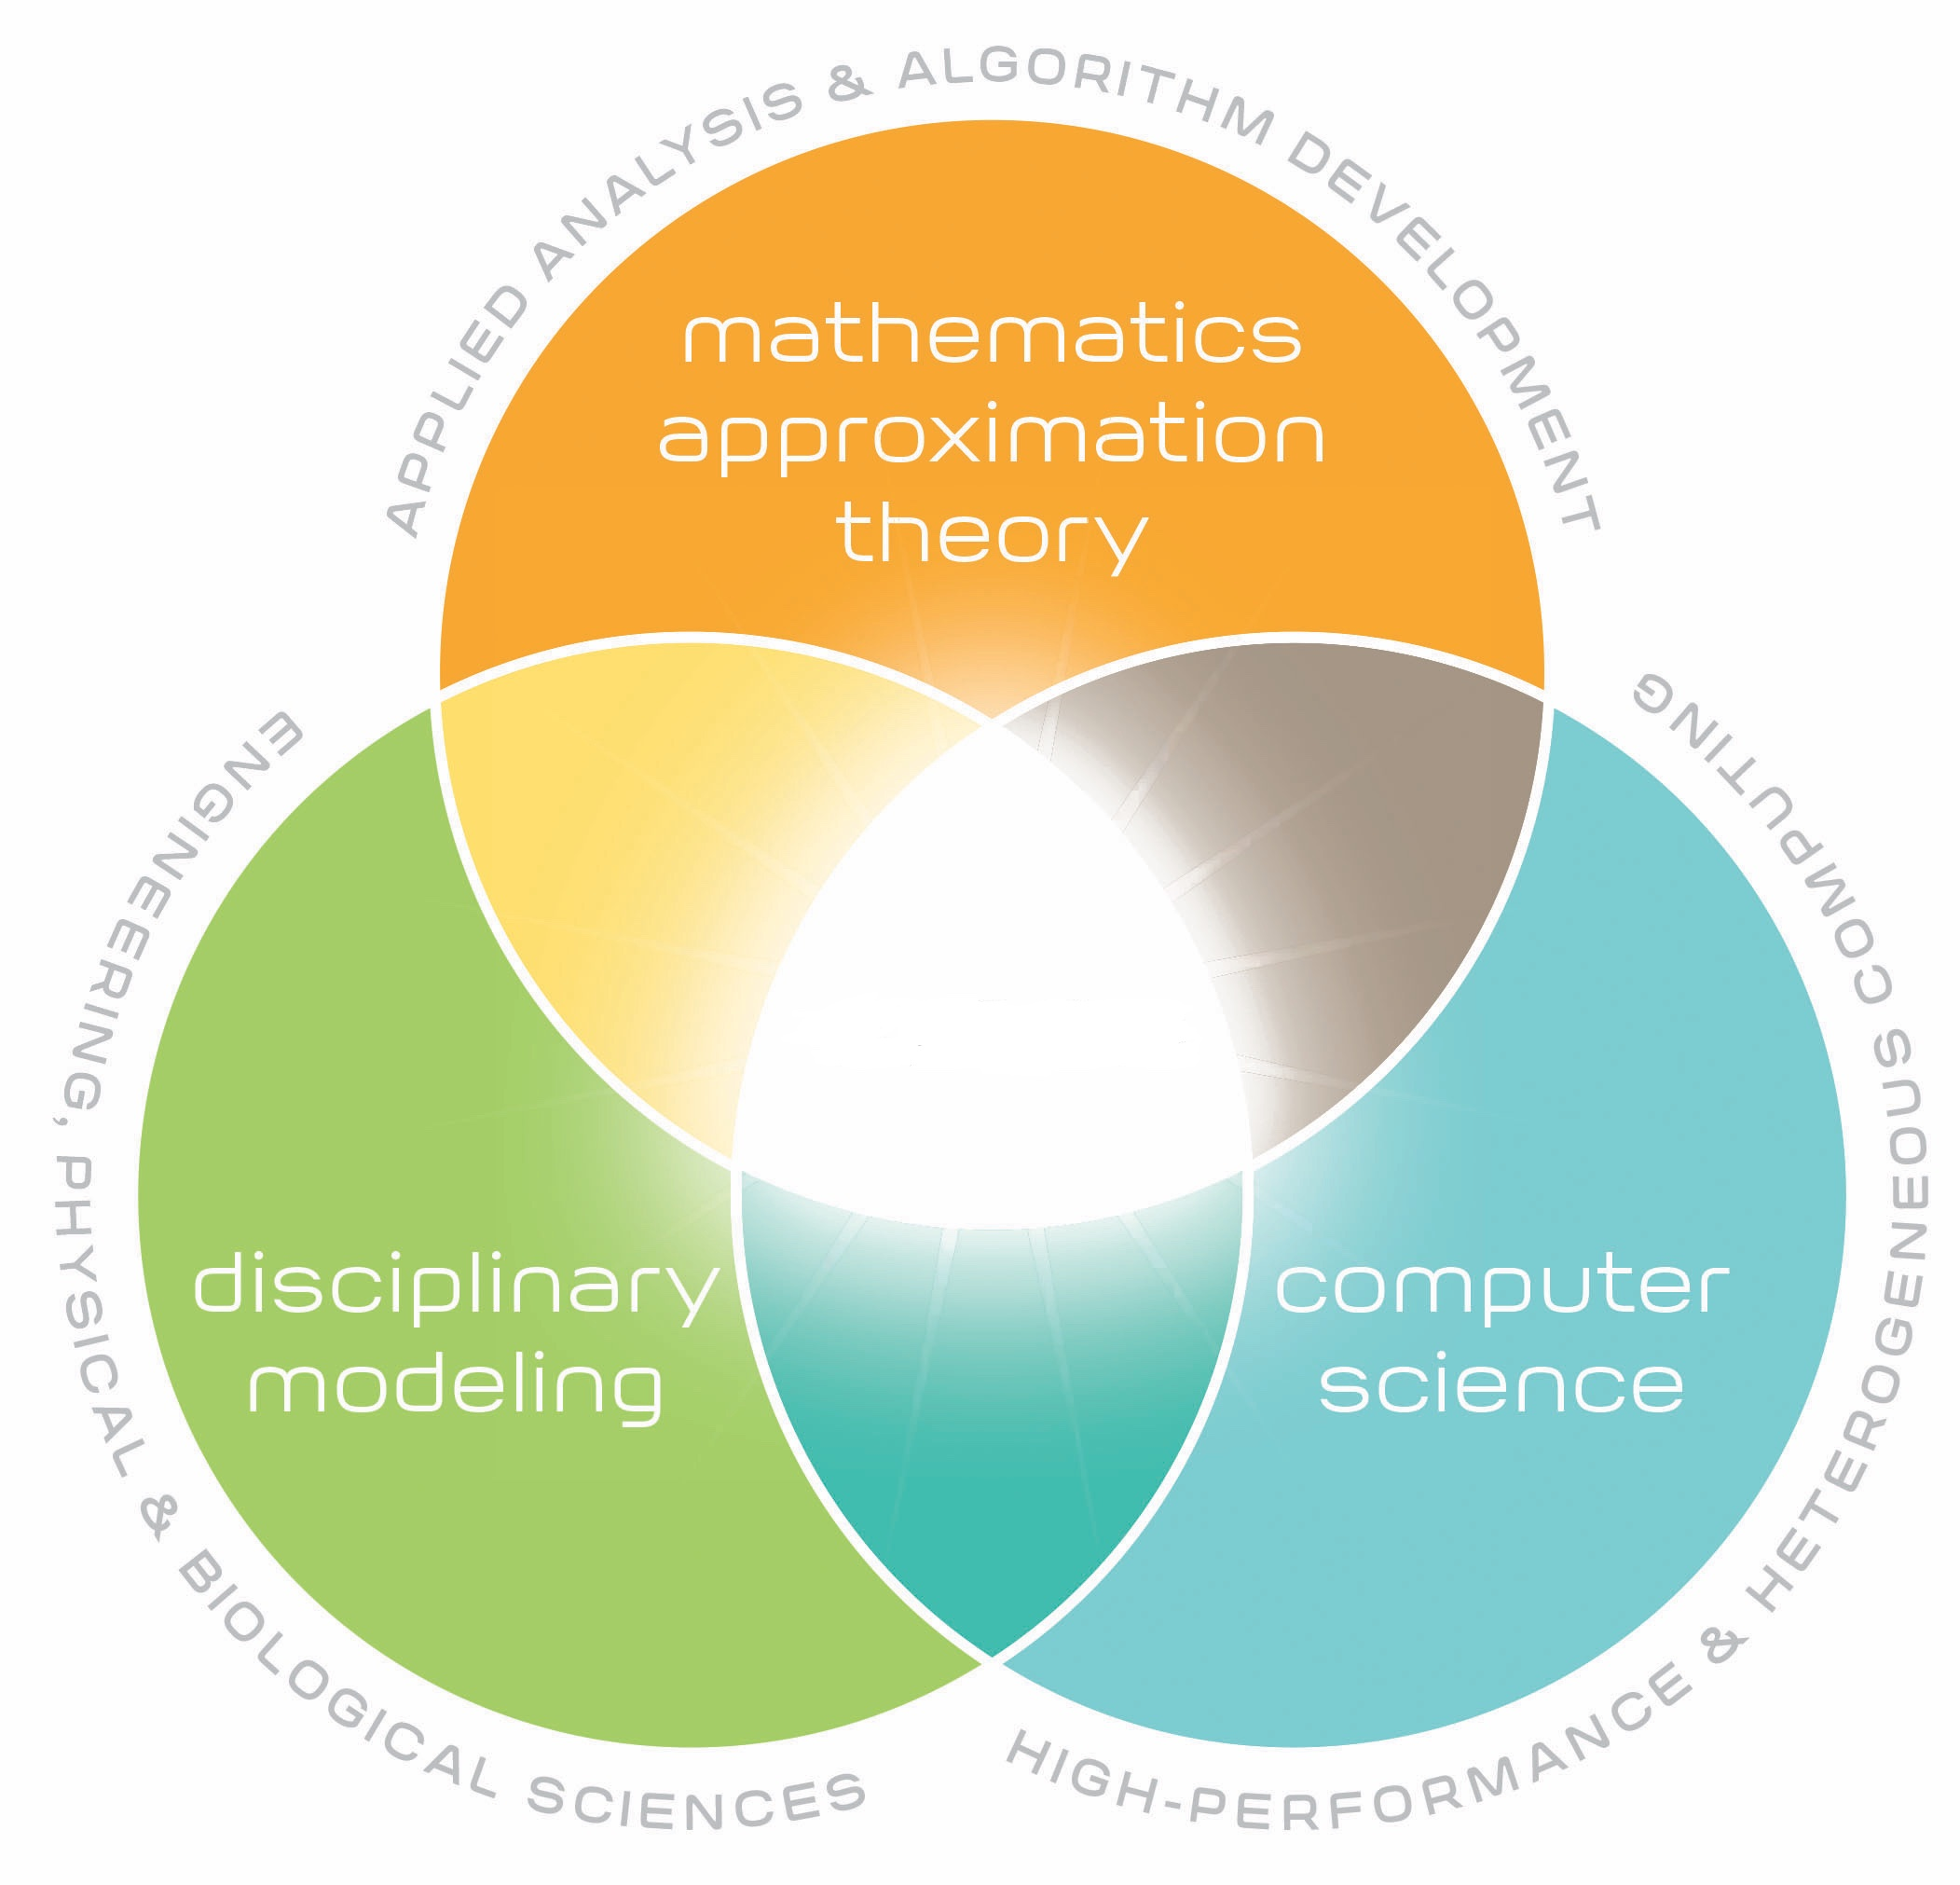
\includegraphics[width=0.7\linewidth]{cs.jpg}}

\vspace{6mm}



\item the foundation for developing joint cutting-edge graduate and undergraduate programs. 
\end{enumerate}


These efforts will open doors to new scientific challenges,
will enable UiO to compete and propose new Center-level funding
opportunities as well as totally new research areas (in the Humanities for example) in computation and data-driven related 
areas that are currently beyond
our reach. It will facilitate the training of scientists and students to be an effective 21st century workforce.  It will also develop courses on modern computational techniques and data modeling that meet the needs of society, both for the public and the private sector. 


We have already developed (starting fall 2018) two new Master of
Science programs, one in \href{{http://www.uio.no/english/studies/programmes/computational-science-master/index.html}}{Computational Science} which includes almost all
disciplines at the MNFak and one on \href{{http://www.uio.no/english/studies/programmes/datascience-master/index.html}}{Data Science}.  These
programs form the basis for our educational efforts that will lead to
an \textbf{across the disciplines PhD program} serving the whole
university. The PhD program will start fall 2020 when the first
students from our two Master of Science program have finalized their
theses.  Based on the two exisiting MSc programs, the new department will research the possibilities of establishing similar MSc programs in Computation and Data Sciences for other disciplines.  Similarly, the new department will aim at establishing similar programs for outside users.  

The new department will coordinate many of its educational
activities with the newly established center of excellence in
education, the Center for Computing in Science Education. It will give
the Computing in Science Education initiative a formal institutional
basis  and together with the Center for Computing in Science Education it
will form a unique powerhouse in educational transformations. The new
department will

\begin{enumerate}
\item Develop a comprehensive set of courses and degree programs at both undergraduate and graduate levels that will give students across the university exposure to practical computational methods, understanding how to analyse data and more generally to the idea of computers as problem-solving tools. The department will also  develop  Software Carpentry and Data Carpentry courses. The courses and the degree programs can also be offered as intensive training courses and programs.	

\item Facilitate the adoption of computational tools and techniques for both research and education across campus, through education and faculty collaboration. A  department will facilitate the pursuit of these goals!	

\item Develop an all university PhD program in Computational Science and Data Science.

\item Based on the new programs (start fall 2018) on Computational Science and Data Sciece, Develop an all university Master of Science Program in Computational Science and Data Science.

\item Develop courses and course modules in Computational Science and Data Science for the private and the public sectors.

\item Develop a Master of Science program and a PhD program in Computational Science and Data Science tailored to the needs of the private and the public sectors, allowing for students residing outside UiO to develop their knowledge about Computational Science and Data Science.

\item Be a driving force in the education of  the next generation of school teachers and university teachers,  with a strong focus on digital competences. 
\end{enumerate}

The department will also have fully developed  our graduate and undergraduate curriculae
with the addition of Bachelor’s programs in computational modeling and
data science, and will have strong enrollment numbers in all education programs. 


The new CDS department  will be unique among computational academic units nationally, the first to comprehensively
treat computation as the triple point of algorithm development and analysis, high performance
computing, and disciplinary knowledge with applications to scientific and engineering modeling
and data science. There is no such department in Norway and very few ones in Europe and Northern America. 
The above paradigm shift recognizes computation as a new discipline rather
than decomposed into isolated sub-disciplines, enabling application-driven computational
modeling and data-driven discoveries, while also exposing disciplinary computationalists to advanced tools and
techniques, which will ignite new transformational connections in research and
education. This research nexus also gives rise to the educational opportunities driven by similar
synergy, leveraging common resources among disciplines, and enabling joint programs and
unique degrees across the entire computational space.



\subsection*{Why should we focus on developing a department in Computational and Data Sciences?}

Modern problems in science and engineering bridge a vast range of temporal and spatial scales
and include a wide variety of physical processes. The analysis of such problems is not possible, so
one must turn to computation. To develop computational tools for such complex systems that
give physically meaningful insights requires a deep understanding of approximation theory, high
performance computing, and domain specific knowledge of the area one is modeling. National laboratories like \href{{https://www.simula.no/}}{SIMULA research lab} have addressed the interdisciplinary nature of computing by having experts
in numerical algorithms co-located with disciplinary experts who have a deep understanding of
computation, and who use scientific computing to address key topics in science.

The proposed organization with  algorithmic scientists and disciplinary scientists in STEM fields as well as other  fields is what facilitates the exploration of challenging multi-disciplinary and
interdisciplinary topics that could not otherwise be addressed. This key observation motivates
the model for the proposed department - a place where we will attack the critical problems
facing us in the 21st century, problem which require the development of computing skills across disciplines, from the traditional STEM fields to the Humanities, Law, Educational Science  and the Social Sciences. 
Furthermore, this department would strive to use
computing as a critical tool to explore fundamental scientific questions in subjects as diverse as
the physics of specific materials, evolutionary biology and data-driven economic forecasting. In addition, the synergy of data-driven computational
modeling, combining aspects of traditional scientific computing with data science and data
mining, is an exciting topic that this new unit will be uniquely suited to address. This is a rapidly
emerging field that touches many of the STEM disciplines but also Medicine, Education, the Humanities and the Social Sciences, and attracting world-leading talent in
this area is greatly facilitated by the introduction of the nurturing environment of the CDS department. Furthermore, the development of the Department of Computational and Data Sciences
has the potential to  catapult UiO into the position of being a
leader in this critical new field, and will open doors to new scientific challenges as well
as new Center-level funding opportunities.

To jump-start this new department at the ‘triple point’ of mathematics, computer science and
discipline-specific computation, we propose recruiting faculty who are experts in numerical
algorithms as well as those whose primary focus is the use of advanced computation to solve a
wide range of challenging scientific problems. 
Furthermore, we wish to define scientific projects where data-driven discovery can play a major role in future years.
In addition, we wish to recruit scientists - having
joint appointments with other units at UiO - whose expertise in computation on heterogeneous
and/or distributed computing platforms, such as hardware-accelerated computing (e.g., GPU
computing), cloud computing, and middleware for dynamic optimization across HPC
architectures. To provide a critical mass, we propose hiring 25 to 30 new faculty across the
aforementioned disciplines. Colocation and research and curriculum ties enable the CDS department  to
break down historical disciplinary boundaries, and become the synergistic leading-edge center
of computational activities on campus. Furthermore, colocating these scientists will enhance
the development of new computational algorithms to address pressing scientific and societal needs and
enable the creation and deployment of the robust numerical tools required for the pursuit of
leadership-class science in virtual laboratories.
Most importantly, the new department will enable new science through these unique interdisciplinary collaborations and will
become a focal point for computational research at UiO, bringing researchers in
computational and data sciences together with domain experts in astrophysics, bioinformatics, chemistry, geoscience
neuroscience, subatomic physics, materials science, life science, the Humanities, economy, Education  and many more.






\paragraph{Strengths, Possibilities and Synergies.}
The University of Oslo has within several of the STEM fields strong research and educational activities, exemplified through for example:
\begin{itemize}
\item Several Centers of excellence in research where Computational Science plays a major role

\item A newly established center of excellence in education research

\item Newly established Master of Science programs in Computational Science and Data Science

\item Several excellent groups in STEM fields that do Computational Science and Data Science

\item Computational topics are included in all undergraduate STEM programs, with the possibility to develop a bachelor program in Computational Science and Data Science for all university colleges

\item Several educational prizes and awards related to computational science 

\item Strong links with research laboratories like SIMULA research lab

\item UiO has the potential to develop cross-college educational programs in Computational Science and Data Science, from undergraduate programs to PhD programs that serve also the public and the private sectors

\item The courses to be developed can be offered to train employees and students outside UiO, serving thus the coming needs of for example Machine Learning for the public and the private sectors
\end{itemize}

\noindent
With a department (or center) we have the possibility to really position UiO as the leading Norwegian and perhaps European institution within Computational Science and Data Science.



\paragraph{Enhance Computational Science and Data Science across the disciplines.}
Data driven discovery and data driven modeling play already a central role in research. The global objective here is to strengthen and coordinate such activities by bringing together scientists and students across the disciplines.
UiO has already strong computational research and education activities within Mathematics and the Natural Sciences.
The aim here is to extend this to include

\begin{itemize}
\item Computational Science and Data Science in Mathematics and all of the physical sciences (Astrophysics, Chemistry, Geoscience and Physics)

\item Bioinformatics

\item Develop research programs in \href{{https://www.aps.org/publications/apsnews/201802/ostp.cfm?utm_source=APS+Physics+Main+Group&utm_campaign=fb7a2e7d6b-News+021218&utm_medium=email&utm_term=0_825303224b-fb7a2e7d6b-106513221}}{Quantum Computing and Quantum Information theory}. Many universities are now developing research and \href{{https://vprgs.msu.edu/event/interdisciplinary-forum-quantum-information-science}}{educational strategies in Quantum Computing}

\item Develop data-driven discovery research programs utilizing recent developments in machine learning

\item Computational life science

\item Computational Materials Science

\item Computational Economy and Data Science and computing in Law and the Social Sciences

\item Data Science and computing in the Humanities
\end{itemize}

\noindent
The new department will host and coordinate research and educational programs in Computational Science and Data Science. In particular research and education that involve  data analysis and Machine Learning will play a central role here. Similarly, the new department will be responsible for developments in quantum computing and quantum information theories. 

\subsection*{Courses and degree programs}

Creation of a robust, coherent set of undergraduate and graduate degrees, with accompanying
courses, supports two complementary goals. First, a coherent program will allow the university
to consolidate undergraduate and graduate training in computation in the STEM fields as well as introducing computing to other disciplines, reducing
redundancy in the courses taught and allowing the university to offer a wider range of more
specialized advanced courses. Second, we will create a robust set of degrees that are designed to give our 
students a strong introduction to computing
that will complement UiO’s existing disciplinary training, and which will make them better suited
to be a part of the workforce in the 21st century, but also to be able to develop and use computing and data Science across the disciplines. These programs will include:
\begin{enumerate}
\item An undergraduate program in Computational and Data Sciences tailored to various disciplines.

\item We have already (from fall 2018) two new Master of Science programs in Computational Science and Data Science dailored to STEM fields. The aim is to extend these to other colleges.

\item Develop a cross-college PhD program in Computational Science and Data Science.

\item Develop courses and course modules in Computational Science and Data Science for the private and the public sectors.

\item Develop a Master of Science program and a PhD program in Computational Science and Data Science tailored to the needs of the private and the public sectors, allowing for participants residing outside UiO to develop their knowledge about Computational Science and Data Science.

\item Be a driving force in the education of  the next generation of school teachers and university teachers,  with a strong focus on digital competences. 
\end{enumerate}

\noindent
This range of options will allow some number of students to dive deeply into
computation through the degree programs, and will enable a much broader swath of the UiO
population to learn about some aspects of computational and data science through not only the various programs but also through the courses to be developed by the new department. 

One desired result of the creation of these
courses and programs is the foundation of a strong community of students from different
disciplines who use similar techniques to solve a wide range of problems, which will promote
broad, interdisciplinary thinking and will help to raise the visibility of computing throughout the UiO campus. We note that an extra benefit of these educational
efforts is that UiO will become an ideal place to perform research in computational science
education, a topic of critical importance that has thus far received little scholarly attention. The new department will have strong links with the recently established Center for Computing in Science Education. 




\paragraph{Long term goals and sustainability.}
The overall goal of this department is to bring together world-leading
faculty who combine the most important aspects of computation and
disciplinary research, thus enabling cutting-edge interdisciplinary
science and the training of both undergraduate and graduate
students. The department will be economically sustained through the standard base
university funding, as any other department at Norwegian universities. 
However, additional funds will be
realized by the securing for example Center-level funding (as well as many
single- or few-PI grants), as well grants obtained the PIs that sustain graduate
students, post-docs, travel and other associated expenses.  In order
to ensure the success of these efforts, the proposed department must
be financially sustainable. Basic university funding (beyond faculty
and support staff salaries) is necessary to support fellowships for
top graduate students, speaker series and honoraria, visitor support,
hardware purchases, and startup packages.


% inline figure
\centerline{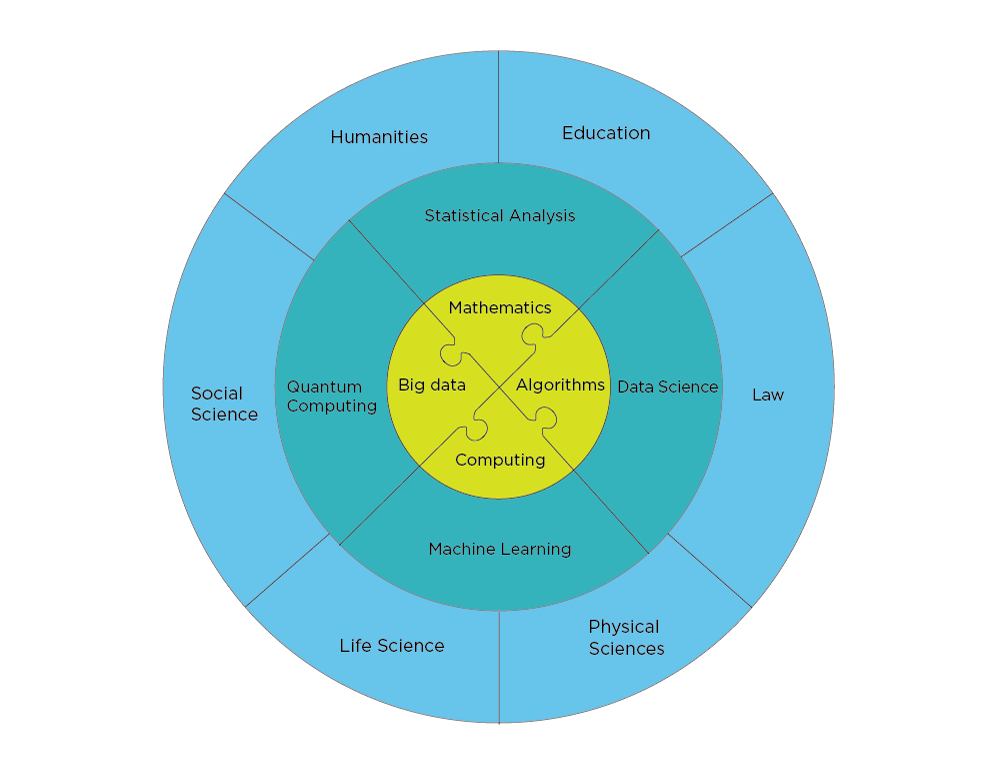
\includegraphics[width=1.0\linewidth]{topics.png}}



\subsection*{Appendix:  Outline of degree programs and courses}

This appendix summarizes the set of degree programs and courses that
can/should be administered by the new department. The range of
offerings gives students the opportunity to engage with computational
science at a variety of levels, from single courses to graduate
programs. Market research and feedback from employers indicate that
engaging with one or more of the proposed programs will substantially
enhance the student's career prospects. The new classes will move to
the new department once the department opens ist doors.

\paragraph{Degree programs.}
The MNFak  offers from fall 2018 two new programs at the Master of Science level in Computational Science and Data Science. These programs are
\begin{enumerate}
\item \href{{http://www.uio.no/english/studies/programmes/computational-science-master/index.html}}{Computational Science}, start fall 2018

\item \href{{http://www.uio.no/english/studies/programmes/datascience-master/index.html}}{Data Science}, start fall 2018

\item Develop similar Master of Science programs tailored to other colleges at UiO, including the Humanities, Law, the Socials Sciences, Medicine and Education by fall 2020

\item Develop an all university PhD program in Computational Science and Data Science by fall 2020

\item Based on these programs and the gained experiences we plan to develop a Master of Science program in Computational Science and Data Science tailored to the needs of the private and the public sectors. This will allow students residing outside UiO to develop their knowledge about Computational Science and Data Science by fall 2021

\item Develop a PhD program in Computational Science and Data Science tailored to the needs of the public and the private sectors (so-called nærings PhD in Norwegian)

\item Develop a bachelor program in Computational Science and Data Science by 2021
\end{enumerate}

\noindent
The Master of Science and PhD programs that will target students from outside UiO (from partner companies, public and private sectors)
will be developed in close collaboration with external stake holders. 

\paragraph{Courses.}
There are several existing and planned courses which could be offered by the new department.
These are
\begin{enumerate}
\item FYS-STK4155 Applied Data Analysis and Machine Learning  (first time fall 2018)

\item IN4230 High-Performance Computing  (first time spring 2019)

\item MAT4110 Computational Mathematics

\item FYS4150 Computational Physics

\item New courses on advanced data analysis and machine learning including for example
\begin{itemize}

  \item Supervised and unsupervised machine learning

  \item Data analysis and machine learning tailored to the Humanities

  \item Data analysis and machine learning tailored to the Social Sciences

  \item Data analysis and machine learning applied to Education programs

  \item Data analysis and machine learning applied to Law 

\end{itemize}

\noindent
\item Multi-particle methods for the Physical Sciences and Life Science

\item Courses on quantum computing and quantum information theory

\item Courses on computations in economy

\item Courses on software carpentry and data carpentry

\item ....
\end{enumerate}

\noindent
Many of these courses, if properly modularized, can be offered as intensive training courses and programs. In particular, such courses will be attractive for both the private and public sectors. The following courses could be offered
\begin{enumerate}
\item Introductory Scientific Python

\item Advanced Scientific Python

\item Data Science and visualization

\item Applied numerical mathematics

\item Computational finance

\item Big data graph analysis

\item Supervised machine learning with scikit-learn and TensorFlow

\item Unsupervised machine learning with scikit-learn

\item Data-driven entrepreneurship

\item Courses tailored to the needs of specific companies

\item and more specialized modules
\end{enumerate}


\end{document}

